\subsection{RAID 4}

RAID 4 combina el funcionamiento de RAID 0 a nivel de bloques, pero añade un disco adicional dedicado para almacenar la paridad, logrando un equilibrio entre rendimiento y tolerancia a fallos.

En este esquema, los datos se distribuyen entre varios discos, como en RAID 0, pero además existe un disco adicional que almacena información de paridad. La paridad permite reconstruir los datos de un disco si este falla.

Por ejemplo, con dos discos de datos y uno de paridad (Figura \ref{fig:raid4}):

\begin{figure}[!ht]
  \centering
  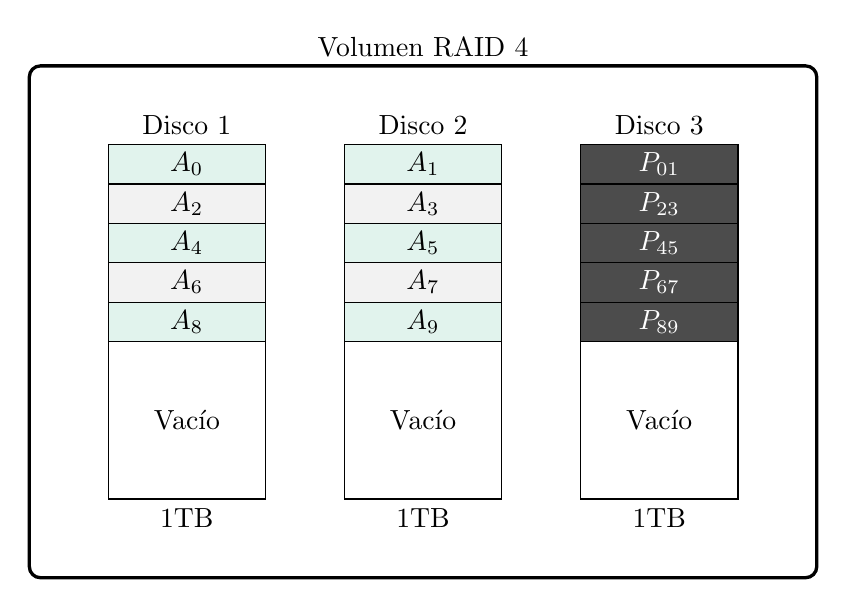
\begin{tikzpicture}
    \node[above] at (1,2.5) {Disco 1};
    \foreach \y\t\c in {
        0/8/white!95!blue!93!green,
        0.5/6/gray!10,
        1/4/white!95!blue!93!green,
        1.5/2/gray!10,
        2/0/white!95!blue!93!green}{
      \draw[fill=\c] (0,\y) rectangle node{\(A_\t\)} (2,{0.5+\y});
    }
    \draw (0,0) rectangle node{Vacío} (2,-2);
    \node[below] at (1,-2) {1TB};

    \node[above] at (4,2.5) {Disco 2};
    \foreach \y\t\c in {
        0/9/white!95!blue!93!green,
        0.5/7/gray!10,
        1/5/white!95!blue!93!green,
        1.5/3/gray!10,
        2/1/white!95!blue!93!green}{
      \draw[fill=\c] (3,\y) rectangle node{\(A_\t\)} (5,{0.5+\y});
    }
    \draw (3,0) rectangle node{Vacío} (5,-2);
    \node[below] at (4,-2) {1TB};

    \node[above] at (7,2.5) {Disco 3};
    \foreach \y\t in {
        0/89,
        0.5/67,
        1/45,
        1.5/23,
        2/01}{
      \draw[fill=black!70] (6,\y) rectangle node[white]{\(P_{\t}\)} (8,{0.5+\y});
    }
    \draw (6,0) rectangle node{Vacío} (8,-2);
    \node[below] at (7,-2) {1TB};

    \draw[very thick,rounded corners] (-1,-3) rectangle (9,3.5);
    \node[above] at (4,3.5) {Volumen RAID 4};
  \end{tikzpicture}
  \caption{Tamaño del volumen de RAID 4: 2TB.}
  \label{fig:raid4}
\end{figure}
Donde:
\begin{itemize}
  \item \(P_{01}\) es la paridad de los bloques \(A_0\) y \(A_1\),
  \item \(P_{23}\) es la paridad de los bloques \(A_2\) y \(A_3\),
  \item \(P_{45}\) es la paridad de los bloques \(A_4\) y \(A_5\) y así sucesivamente.
\end{itemize}
La paridad suele calcularse mediante la operación XOR:
\[
  P_{01} = A_0 \oplus A_1
\]
Si, por ejemplo, falla el Disco 2, el bloque perdido puede recuperarse usando:
\[
  A_1 = P_{01} \oplus A_0
\]
Y en caso de tener más de dos discos de datos, la paridad es simplemente la operación XOR entre todos los discos:
\[
  P = A_0 \oplus A_1 \oplus \cdots \oplus A_n
\]

\paragraph{Ventajas:}
\begin{itemize}
  \item Tolera la falla de un disco sin perder información.
  \item Las lecturas son rápidas, ya que los datos están distribuidos entre varios discos.
  \item Aprovecha mejor la capacidad que RAID 1.
\end{itemize}

\paragraph{Desventajas:}
\begin{itemize}
  \item Todas las escrituras deben actualizar el disco de paridad, lo que lo convierte en un cuello de botella.
  \item El rendimiento en escritura disminuye cuando hay muchas escrituras concurrentes.
\end{itemize}

\paragraph{¿Por qué RAID 4 casi no se utiliza?}

El principal problema es el disco de paridad dedicado. En cargas con muchas escrituras, ese disco debe actualizarse constantemente y termina limitando el rendimiento del arreglo o fallando por desgaste mecánico.

Por esta razón, en la práctica RAID 5 reemplazó casi por completo a RAID 4, ya que distribuye la paridad entre todos los discos y elimina la desventaja principal. RAID 4 se considera principalmente de interés histórico o académico.

\begin{table}[!ht]
  \centering
  \begin{tabular}{l|c}
    Cantidad de discos mínima & 3 \\\hline
    Cantidad de discos que pueden fallar & 1 \\ \hline
    Velocidad de escritura relativa a un disco & \(\frac{\text{VDisco}}{\text{Cant. Oper.}}\)~[MB/s] \\\hline
    Velocidad de escritura ponderada & 2 \\ \hline
    Velocidad de lectura relativa a un disco & VDisco~[MB/s] \\ \hline
    Velocidad de lectura ponderada & 5 \\ \hline
    Costo & Medio
  \end{tabular}
  \caption{Características del RAID 4.}
\end{table}
